\section{Optimisation for Processor Architectures
\label{sec:pa}}

\subsection{NVIDIA GPU}
The LFRic-microbenchmark suite~\cite{lfric-microbenchmarks} allows
optimisations for individual kernels to be explored without having to
compile and run the whole code. This is particularly useful when
targeting a programming model such as OpenACC for GPU architecture
where the Portland group compiler cannot compile the Fortran 2003 of
the whole code.

The local matrix assembly (LMA) matrix-vector routine had been
previously ported to run on GPUs by inserting OpenACC directives in
the PSy layer code to control the data transfer from host memory to
device memory and to offload the kernel call to the GPU device. This
Open ACC version was given to NVIDIA to look at optimisations. Alan
Gray made several optimisations and sent a report on the improvemnents
achieved.

\begin{figure}
\centering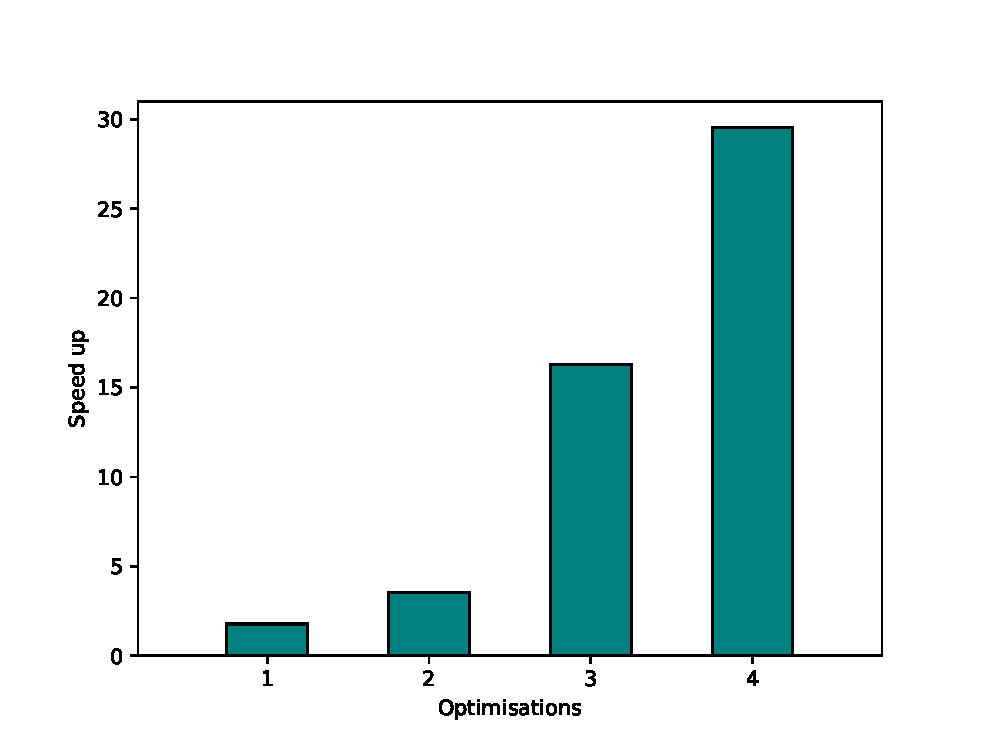
\includegraphics[width=1.0\linewidth]{figs/LMA-nvidia.eps}
\caption{\label{fig:lma_nvidia}Speed up versus original code for
  various optimisations. 1 loop fusion. 2 loop collapse. 3 Inlining. 4
  Single Kernel.}
\end{figure} 



